\documentclass[fontset=none]{ctexart}

\usepackage[T1]{fontenc}
\usepackage{fontspec}
\setCJKmainfont{SimSun}
% Latin Modern
\renewcommand*\ttdefault{txtt} % 改等宽字体

\setcounter{tocdepth}{5}
\setcounter{secnumdepth}{5}
% -1 part
% 0 chapter
% 1 section
% 2 subsection
% 3 subsubsection
% 4 paragraph
% 5 subparagraph

\usepackage{cite}
\usepackage{geometry}
\geometry{a4paper,scale=0.8}

\usepackage{algorithm}  
\usepackage{algorithmicx}  
\usepackage{algpseudocode}
\makeatletter
\newenvironment{breakablealgorithm}
  {% \begin{breakablealgorithm}
   \begin{center}
     \refstepcounter{algorithm}% New algorithm
     \hrule height.8pt depth0pt \kern2pt% \@fs@pre for \@fs@ruled
     \renewcommand{\caption}[2][\relax]{% Make a new \caption
       {\raggedright\textbf{\ALG@name~\thealgorithm} ##2\par}%
       \ifx\relax##1\relax % #1 is \relax
         \addcontentsline{loa}{algorithm}{\protect\numberline{\thealgorithm}##2}%
       \else % #1 is not \relax
         \addcontentsline{loa}{algorithm}{\protect\numberline{\thealgorithm}##1}%
       \fi
       \kern2pt\hrule\kern2pt
     }
  }{% \end{breakablealgorithm}
     \kern2pt\hrule\relax% \@fs@post for \@fs@ruled
   \end{center}
  }
\makeatother

\usepackage{amsmath}
\usepackage{amssymb}
\usepackage{graphicx}
\usepackage{subfigure}
\usepackage{changepage}
\usepackage{multirow}
\usepackage{url}

\usepackage{amsthm}
\newtheorem{theorem}{Theorem}[section]
\newtheorem{lemma}[theorem]{Lemma}
\newtheorem{proposition}[theorem]{Proposition}
\newtheorem{corollary}[theorem]{Corollary}
% \newtheorem{remark}{Remark}[section]
\newtheorem{example}{Example}[section]
\newenvironment{solution}{\begin{proof}[Solution]}{\end{proof}}
\theoremstyle{definition}
\newtheorem{definition}{Definition}[section]
\theoremstyle{remark}
\newtheorem*{remark}{Remark}

\usepackage[colorlinks, linkcolor=black, citecolor=blue, bookmarksnumbered]{hyperref}
% \hypersetup{
% 	colorlinks=true,
% 	linkcolor=cyan,
% 	filecolor=blue,      
% 	urlcolor=red,
% 	citecolor=green,
% }

\usepackage{fancyhdr}
\pagestyle{fancy}
\renewcommand{\sectionmark}[1]{\markright{\thesection\ #1}}
\fancyhf{}
\cfoot{\thepage}
\lhead{\rightmark}
% \rightmark 当前的节名
% \leftmark 当前的章名
% \(l/c/r)head{}, \(l/c/r)foot{}
\renewcommand{\headrulewidth}{0.4pt}
\renewcommand{\footrulewidth}{0pt}

\renewcommand\refname{References}
\renewcommand\contentsname{Contents}
\renewcommand\figurename{Figure}

\begin{document}

\begin{titlepage}
    \begin{center}
        \vspace*{1cm}
            
        \Huge
        \textbf{Traffic Network Flow\\ Estimation Based On\\ Social Network Influence Model}
            
        \vspace{0.5cm}
        \LARGE
        Final Report\\
            
        \vspace{1.5cm}
            
        \textbf{11812804}  董\quad 正\\
        \textbf{11810419}  王焕辰\\
        \textbf{11811305}  崔俞崧\\

        \vspace{0.5cm}
        Supervisior: 宋轩
            
        \vfill
            
        
\includegraphics[width=\textwidth]{images/sustc.png}
            
        \vspace{0.2cm}
            
        \Large
        Department of Computer Science and Engineering\\
        \vspace{0.5cm}
        Jan. 2022
            
    \end{center}
\end{titlepage}

\tableofcontents

\clearpage
\section{Preliminaries}
\subsection{Review}
In this semester, we will try to build a traffic flow estimation system based on graph neural network and
social network influence model. We have changed the system design a little.
Currently, the structure of the whole system is

\begin{figure}[htb]
  \centering
  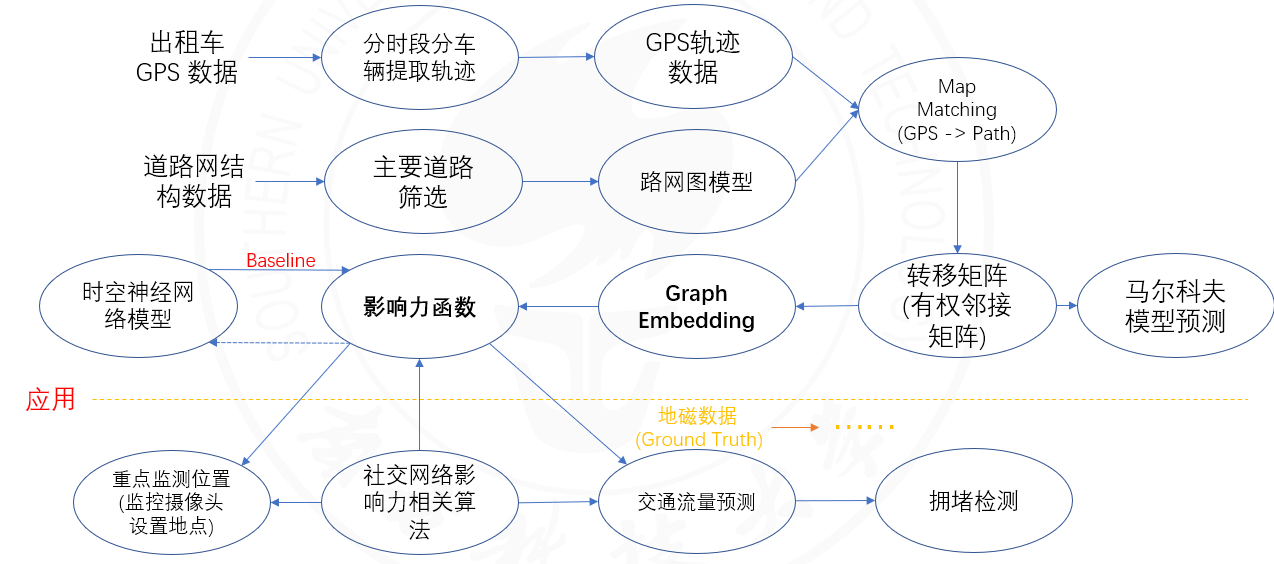
\includegraphics[width=\textwidth]{images/8-1-1.png}
  \caption{System Structure}
  \label{fig: structure}
\end{figure}

\begin{enumerate}
  \item Process taxi GPS data to get tracks
  \item Process road network data to get a basic graph model
  \item Match tracks to each road and get the adjacent matrix of the graph
  \item Try a simple prediction based on Markov model
  \item \textbf{Graph embedding}
  \item \textbf{Influence function design}
  \item Combine spatial-temporal models and use them as baseline
  \item Combine social network influence algorithms to predict traffic network flow, use geomagnetic data as one of the ground truth
  \item Applications: traffic surveillance camera position and traffic jam detection
\end{enumerate}

\subsection{Report Contents}
Breifly, we will state our work in this report as
\begin{itemize}
  \item AAAI21: Traffic Flow Prediction with Vehicle Trajectories 董正 \& 崔俞崧
  \item LibCity Exploring 董正 \& 崔俞崧
  \item Geomagnetic data Network Construction \& Basic regression Prediction 王焕辰
\end{itemize}

\clearpage
\section{AAAI21: Traffic Flow Prediction with Vehicle Trajectories}
In this part, we will introduce a paper in AAAI\cite{MingqianLi2021TrafficFP} whose work is very similar to ours.
What's more, we will make a comparsion on design ideas between thier and ours.

\subsection{Trajectory Transition}
\begin{itemize}
  \item Model trajectory transition as a Markov process.
  \item Calculate transition matrix for each time interval, the design and calculation process is exactly same as ours.
  \item However, $1^{st}$ order transition matrix cannot capture high-dimensional transition information.
        Therefore, we decided to use graph embedding on trajectory.
\end{itemize}
\begin{figure}[htb]
  \centering
  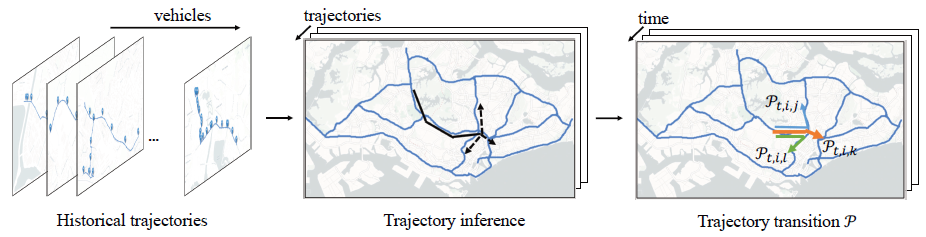
\includegraphics[width=\textwidth]{images/9-1-1.png}
  \caption{Trajectory Transition Model}
  \label{911}
\end{figure}

\subsection{Traffic Demand}
For spatial modeling, they use graph propagation from Graph Convolutional
Networks to simulate the transition of
vehicles along the road network. Then perform graph propagation
in $d$ hops, resulting in a graph of traffic demand for
each hop. For each input time interval $t$, the traffic demand is
\begin{equation}
  D_t=GraphProp(X_t, \mathcal P_t^T;d)
  =[X_t||\mathcal P_t^TX_t||(\mathcal P_t^T)^2X_t||\dots||(\mathcal P_t^T)^dX_t]
  \notag
\end{equation}
As we can see, it is a Markov propagation.

For temporal modeling, they use traffic status for attention.
Traffic status refers to the
overall traffic volume in the neighboring of each road segment.
If the traffic status is congested around a road segment
(i.e., high volume of flows in the neighboring road
segments), the propagation of flows along that road segment
should be slow, and vice versa.

For each time interval, they applied bidirectional graph propagation method 
to get current traffic statusof each neighbor.

\clearpage
\begin{figure}[htb]
  \centering
  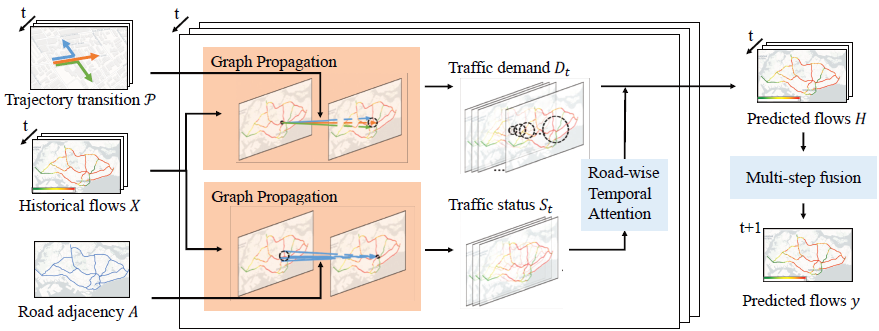
\includegraphics[width=\textwidth]{images/9-1-2.png}
  \caption{Model Structure}
  \label{912}
\end{figure}

\subsection{Performance}
\begin{figure}[htb]
  \centering
  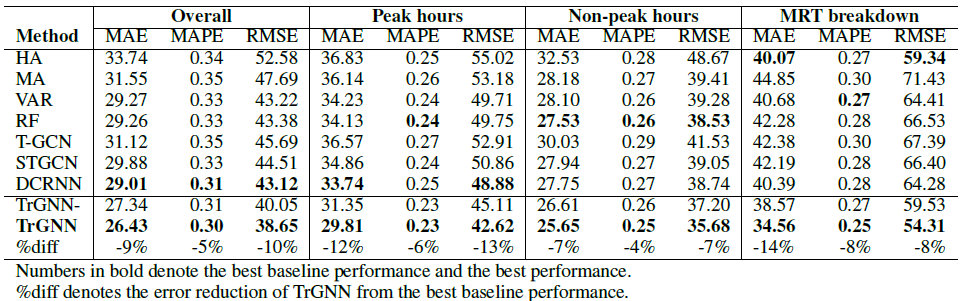
\includegraphics[width=\textwidth]{images/9-1-3.png}
  \caption{Performance}
  \label{913}
\end{figure}
As we can see, this model achieves a much better result than SOTA GCNs.
However, the baseline models, i.e. T-GCN, STGCN and DCRNN are designed for speed prediction.
We doubt that why the author did not choose flow prediction models.

\subsection{Preprocessing}
For raw GPS data, the author applied these methods to convert it to flow data:
\begin{enumerate}
  \item Map Matching: Hidden Markov Map Matching (HMMM)

        HMMM maps a whole trajectory to road network and needs road connectivity information.
  \item Trajectory Split
        \begin{itemize}
          \item GPS is off for over 10 minutes
          \item Driver stay on same road for 2 minutes
          \item No path between two consecutive GPS points
        \end{itemize}
  \item Trajectory Recovery
  \item 
        For each two consecutive GPS points, run Dijkstra algorithm to find shortest path.
  \item Flow Aggregation: aggregate on 15 minutes time interval
\end{enumerate}

The preprocessing methods are worthy to learn, thus, we applied many similar procedure when process our data.

\clearpage
\section{LibCity Exploring}
LibCity\cite{10.1145/3474717.3483923} is a unified, comprehensive, and extensible library, which provides researchers with a credible experimental tool and a convenient development framework in the traffic prediction field.
\begin{figure}[htb]
  \centering
  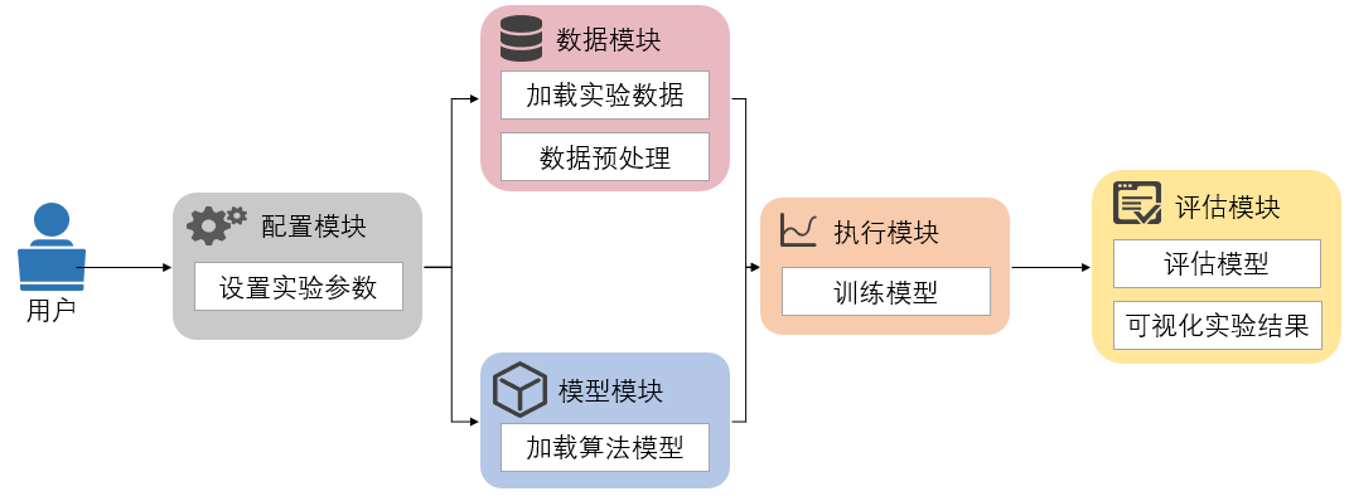
\includegraphics[width=\textwidth]{images/9-2-1.png}
  \caption{LibCity Structure}
  \label{921}
\end{figure}

\subsection{Atomic Files}
Atomic files are \texttt{.csv} files defined by LibCity. Every raw data should be converted to these atomic files,
which gurantees the uniformity of different raw data.

\begin{table}[!ht]
  \centering
  \begin{tabular}{|l|l|}
  \hline
      \textbf{Filename} & \textbf{Content} \\ \hline
      \texttt{xxx.geo} & Store geographic entity attribute information. \\ \hline
      \texttt{xxx.usr} & Store traffic user information. \\ \hline
      \texttt{xxx.rel} & Store the relationship information between entities, such as road networks. \\ \hline
      \texttt{xxx.dyna} & Store traffic condition information. \\ \hline
      \texttt{xxx.ext} & Store external information, such as weather, temperature, etc. \\ \hline
      \texttt{config.json} & Used to supplement the description of the above table information. \\ \hline
  \end{tabular}
\end{table}

The core file is \texttt{.dyna} which stores traffic state data for traffic prediction, or
trajectory data for map matching.

\subsection{LibCity Map Matching}
The matching model we chose is HMMM.
\begin{enumerate}
  \item Convert raw GPS data to atomic files.
        \begin{itemize}
          \item \texttt{.geo}: Road ID and geometry information.
          \item \texttt{.rel}: Adjacency list.
          \item \texttt{.usr}: Taxi ID.
          \item \texttt{.dyna}: Trajectories, where we applied trajectory split methods.
          
          \begin{table}[!ht]
            \centering
            \begin{tabular}{|l|l|l|l|l|l|}
            \hline
                dyna\_id & type & time & entity\_id & traj\_id & coordinates \\ \hline
                0 & trajectory & 2019-12-02T00:10:30Z & 15876 & 0 & [114.06776, 22.550152] \\ \hline
                1 & trajectory & 2019-12-02T00:11:32Z & 15876 & 0 & [114.06859, 22.54198] \\ \hline
                2 & trajectory & 2019-12-02T00:12:12Z & 15876 & 0 & [114.07125, 22.542738] \\ \hline
                3 & trajectory & 2019-12-02T00:51:17Z & 15876 & 1 & [114.04781, 22.539036] \\ \hline
                4 & trajectory & 2019-12-02T00:51:47Z & 15876 & 1 & [114.04774, 22.538887] \\ \hline
                ... & ... & ... & ... & ... & ... \\ \hline
                95 & trajectory & 2019-12-02T15:43:25Z & 15876 & 7 & [114.05783, 22.531305] \\ \hline
                96 & trajectory & 2019-12-02T15:51:55Z & 15876 & 7 & [114.05137, 22.53659] \\ \hline
                97 & trajectory & 2019-12-02T15:55:40Z & 15876 & 7 & [114.05117, 22.53749] \\ \hline
                98 & trajectory & 2019-12-02T15:57:38Z & 15876 & 7 & [114.051216, 22.539156] \\ \hline
                99 & trajectory & 2019-12-02T15:59:26Z & 15876 & 7 & [114.05119, 22.545998] \\ \hline
            \end{tabular}
        \end{table}
        \end{itemize}

        However, we also found some shortcomings:
        \begin{itemize}
          \item Lack APIs for \texttt{OSM} and \texttt{NetworkX}.
          \item Different raw data need totally different convert scipts.
          \item \text{.csv} format leads to lots of duplicated information.
          \item Lack of documents.
        \end{itemize}
  \item Run HMMM model.
        \begin{itemize}
          \item It is convenient. If the structure of atomic files are correct, we can run directly by a simple command.
          \item LibCity provides a set of parameters.
          \item LibCity outputs very detailed logs.
        \end{itemize}
        Still, the shortcomings are:
        \begin{itemize}
          \item Bugs in array index, eg. \texttt{while a[k] and k < len(a)-1}.
          \item Does not check \texttt{null} or empty sets.
          \item Wide usage of time-costing functions, eg. \texttt{DataFrame.iterrows()}.
          \item Does not support multithreading.
        \end{itemize}
\end{enumerate}

\subsection{Traffic Flow Prediction Baseline}
\begin{enumerate}
  \item Convert matched trajectory data to \texttt{.dyna} file.

        Here we used the data for calculating transition matrix and graph embedding in our last report.

        It contains 16153 roads, and the spatial range is whole Shenzhen, the time range is Mon. to Fri.
  \item Flow Aggregation: the time interval is 15min, and 96 intervals per day.
        \begin{table}[!ht]
          \centering
          \begin{tabular}{|l|l|l|l|l|}
          \hline
              dyna\_id & type & time & entity\_id & flow \\ \hline
              0 & state & 2019-12-02T00:00:00Z & 0 & 5 \\ \hline
              1 & state & 2019-12-02T00:00:00Z & 1 & 2 \\ \hline
              2 & state & 2019-12-02T00:00:00Z & 2 & 9 \\ \hline
              3 & state & 2019-12-02T00:00:00Z & 3 & 2 \\ \hline
              4 & state & 2019-12-02T00:00:00Z & 4 & 3 \\ \hline
              ... & ... & ... & ... & ... \\ \hline
              95 & state & 2019-12-02T00:00:00Z & 95 & 0 \\ \hline
              96 & state & 2019-12-02T00:00:00Z & 96 & 0 \\ \hline
              97 & state & 2019-12-02T00:00:00Z & 97 & 0 \\ \hline
              98 & state & 2019-12-02T00:00:00Z & 98 & 1 \\ \hline
              99 & state & 2019-12-02T00:00:00Z & 99 & 0 \\ \hline
          \end{tabular}
      \end{table}
  \item Load model. LibCity auto splits train, vaild and test datasets.
  \item Model training. LibCity uses \texttt{Ray Tune} to adjust parameters automatically.
  \item Model evaluation. LibCity provides many kinds of metrics.
\end{enumerate}

However, the result of our dataset is bad.
We only run simple NNs successfully, and GCNs are out of memory when training because
our road network is too large.

The evaluation for simple NNs are also not good:
\begin{table}[htb]
  \centering
  \begin{tabular}{|c|c|c|c|}
  \hline
      Model & MAE & Masked MAPE & Masked RMSE\\ \hline
      AutoEncoder & 3.13 & 0.79 & 11.57\\ 
      GRU & 5.22 & 2.01 & 12.11\\ 
      LSTM & 3.24 & 0.87 & 11.45\\ 
      FNN & 2.52 & 0.75 & 11.98\\ 
      Seq2seq & 5.44 & 2.1 & 12.66\\
  \hline
  \end{tabular}
\end{table}

\subsection{Future Plan}
\begin{enumerate}
  \item Re-select road network based on raw GPS data. We plan to select about 200~500 roads.
  \item Try only one day's data.
  \item Try to run GCN baseline successfully first, and then enlarge time duration.
\end{enumerate}

\clearpage
\section{Geomagnetic data Network Construction \& Basic regression Prediction}
\subsection{Divide the Area and Build the Road Network}
According to the administrative divisions of Shenzhen and the concentration of traffic flow recorded at each monitoring point, select two regions and divide them.

According to the actual geomagnetic detection points recorded in the data, construct the road connection network map of this region and generate an adjacency matrix.

However, the two areas only take each geomagnetic detection point as the graph node, without considering the inflow and outflow, at present. The adjacency matrix of the road network in Futian District is $34\times34$, with $59$ edges in total.
\begin{figure}[htb]
  \centering
  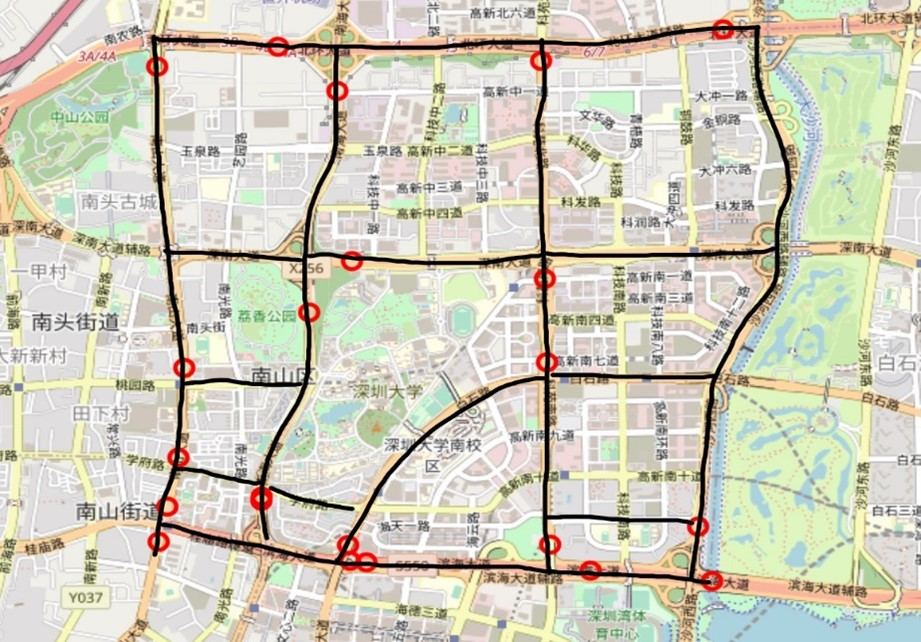
\includegraphics[width=\textwidth]{images/9-3-1.jpg}
  \caption{Nanshan district central road network}
  \label{931}
\end{figure}
\clearpage
\begin{figure}[htb]
  \centering
  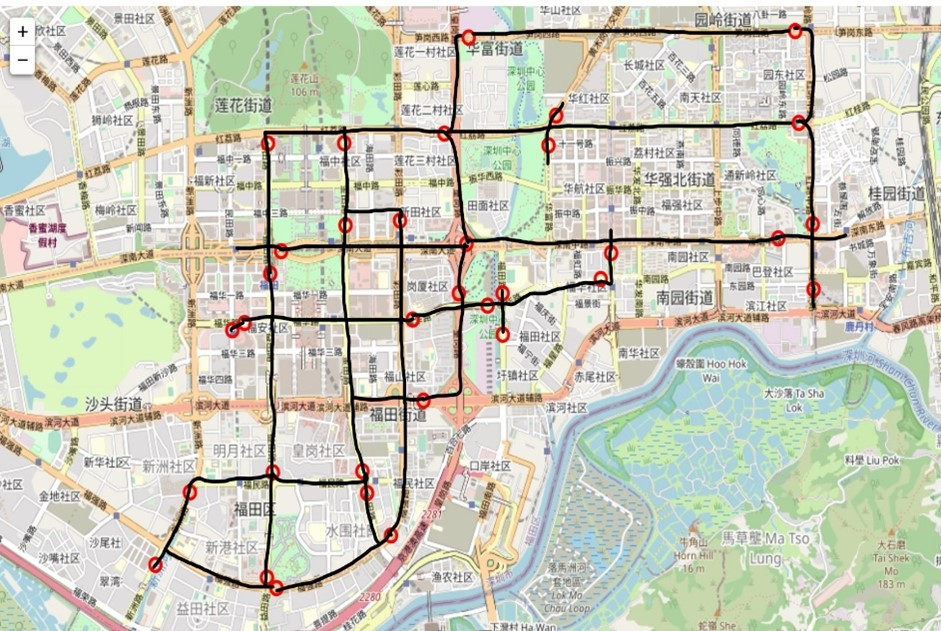
\includegraphics[width=\textwidth]{images/9-3-2.jpg}
  \caption{Futian district central road network}
  \label{932}
\end{figure}

\clearpage
\subsection{Existing Problems in Network Construction}
At present, the matrix only contains connection relation and does not contain lane information. The network is only established by connecting the recorded detection points in the data, without considering lane information and traffic flow direction.  

There are data records of the detection point is only 127, not in conformity with the point description provided in 318, In January 2019 to August 2020 data, it has been found after the preprocessing, which causes the original connection relations of intensive figure and become sparse, have to expand the area (such as Futian area had a smaller area should have 45 points).  At present, we are communicating with Shenzhen Transportation Bureau to find the cause of missing data.
\begin{figure}[htb]
  \centering
  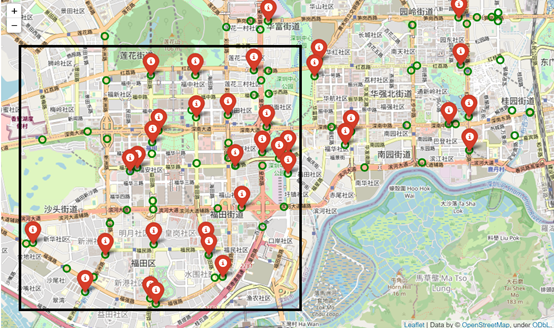
\includegraphics[width=\textwidth]{images/9-3-3.png}
  \caption{Actual points and missing points (green are the missing points)}
  \label{933}
\end{figure}

\clearpage
\subsection{Process Data in Groups by Flow Direction}
After the network construction is completed, the traffic data of each node are grouped according to time and traffic flow for regression prediction to generate both inflow and outflow data. Among the incoming or outgoing data, the traffic of some data is not recorded in all time periods or is not recorded after a certain time period. Considering one-way street and traffic restriction factors after a fixed time period, these NAN values are set to 0.
\begin{figure}[htb]
  \centering
  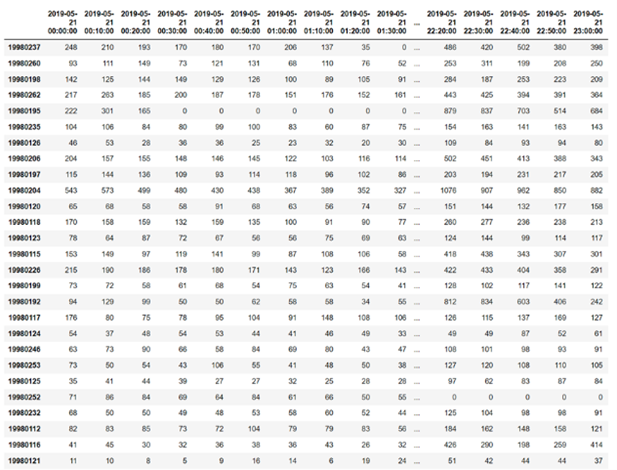
\includegraphics[width=\textwidth]{images/9-3-4.png}
  \caption{Inflow of each road in Futian regional road network}
  \label{934}
\end{figure}

\clearpage
\subsection{Basic Prediction}
Basic prediction of flow data is made through linear regression and random forest, and the results are shown in the table below:
\begin{table}[htb]
  \centering
  \begin{tabular}{|c|c|c|c|}
  \hline
      Model & MAE & MAPE & RMSE\\ \hline
      Random Forest & 37.45 & 0.24 & 58.82\\
      Linear Regression & 46.83 & 0.26 & 74.98\\
  \hline
  \end{tabular}
\end{table}

At present, only two basic models are used and only the inflow and outflow data are segmented for training, without more effective use of spatial data (adjacent matrix). Besides, the LSTM, GRU, and other neural network models will be added later to complete the baseline.

\clearpage
\phantomsection
\addcontentsline{toc}{section}{References}
\bibliographystyle{ieeetr}
\bibliography{references9}

\end{document}